\section{Data Widget}
\label{sec:osgview_data}

\subsection{Mouse/Keyboard Operations}
In the data widget, several mouse and key operations are supported. The following terms are used:

\begin{itemize}
 \item LMB: Left mouse button
 \item MMB: Middle mouse button
 \item RMB: Right mouse button
\end{itemize}

The following operations exist, if no tool is used (from the toolbar):

\begin{table}[H]
  \center
  \begin{tabular}{ | l | l | l | l |}
    \hline
    \textbf{Mouse Action} & \textbf{Clicked element} &\textbf{Key Action} &  \textbf{Description} \\ \hline
    LMB click & Geometry & Label & Toggle label \\ \hline
    LMB click and hold & Label & Label & Maximize label \\ \hline
    LMB click \& drag & & - & Traverse map \\ \hline
    LMB double click & & - & Zoom to clicked location \\ \hline
    - & Arrows & Traverse map \\ \hline
    MMB click \& drag & & - & Rotate map \\ \hline
    MMB scroll \& drag & & - & Zoom map \\ \hline
    RMB click & & Quick menu & Clear labels/selection/measurements \\ \hline
    RMB click & Geometry & Geometry menu & Various actions \\ \hline
    RMB click \& drag & & - & Zoom map \\ \hline
    - & & Space bar & Return to home position \\ \hline
  \end{tabular}
  \caption{Map widget view operations in Navigate mode}
\end{table}

Different operations exist depending on what is clicked.

\subsection{Status Information}
%DONE

In the lower-left corner, the data status information is given:

\begin{itemize}
 \item Begin: First timestamp in the data, in YYYY-MM-DD HH:MM:SS
 \item End: Last timestamp in the data, in YYYY-MM-DD HH:MM:SS
 \item Loaded: Number of loaded target reports (from the database)
 \item Skipped: Number of not-drawn target reports
 \item Drawn: Number of drawn target reports
 \item Selected: Number of selected target reports
\end{itemize}
\  \\

In the upper-right corner, the COMPASS version is shown. %In the lower-right corner, the current coordinates (map coordinates under the mouse cursor) are shown. 

\subsection{Data Operations}

\subsubsection{Data Labeling}

Labels can be shown for target reports. Simply do a LMB click on a target report symbol.

\begin{figure}[H]
    \hspace*{-2.5cm}
    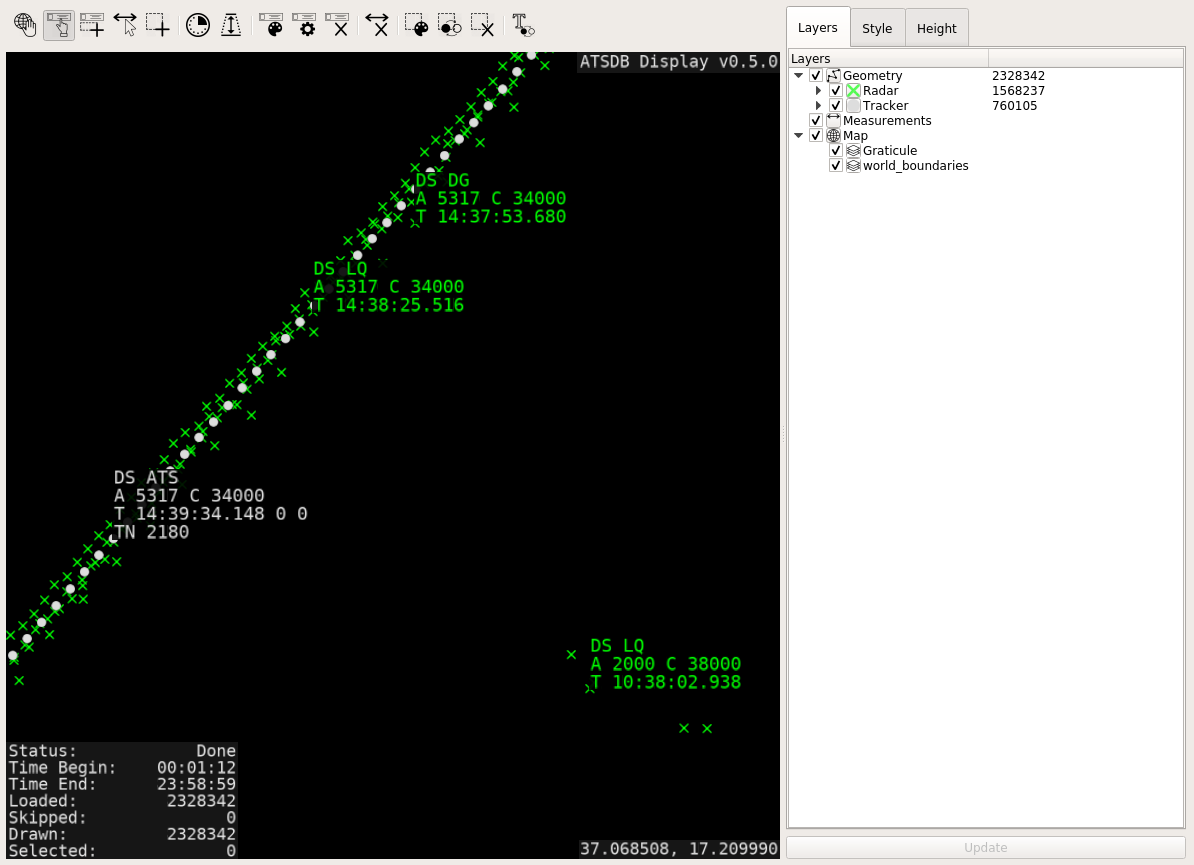
\includegraphics[width=19cm,frame]{figures/osgview_labels.png}
  \caption{OSG View Labels}
\end{figure}

Please note that if automatic labeling is active, manually created labels are cleared every 1 second. This will be improved in a future version.

\subsubsection{Maximized Label}

Existing labels can be maximized to show all (currently available) information about a target report. Simply do a LMB click on a existing label and hold the LMB.

\begin{figure}[H]
    \hspace*{-2.5cm}
    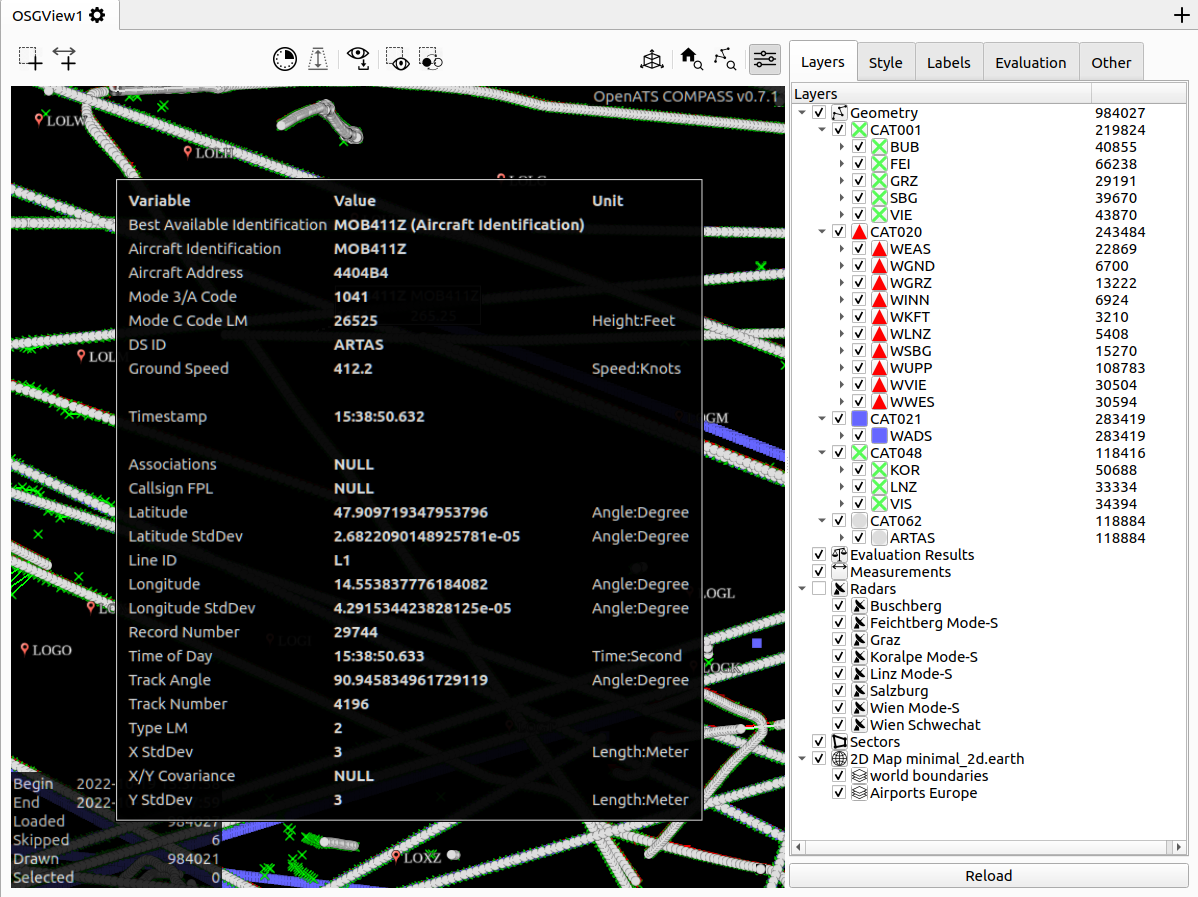
\includegraphics[width=19cm,frame]{figures/osgview_max_label.png}
  \caption{OSG View maximized label}
\end{figure}

The maximized label information is shown until the LMB is released.

\subsubsection{Geometry Menu}

Several data-related operations can be performed in the data widget by a RMB click on a target report symbol.

\begin{figure}[H]
    \hspace*{-2.5cm}
    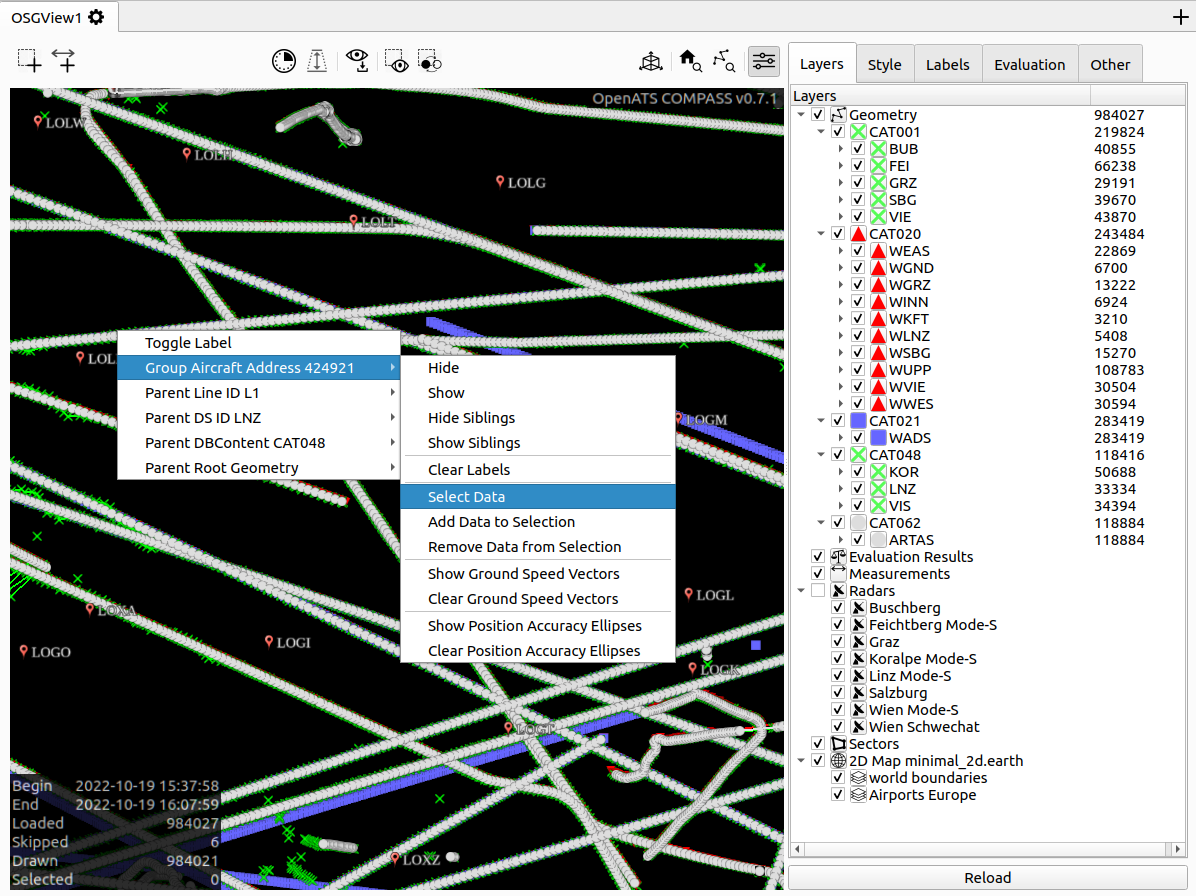
\includegraphics[width=19cm,frame]{figures/osgview_data_operations.png}
  \caption{OSG View geometry operations}
\end{figure}

The data context menu allows the following operations:

\begin{itemize}
 \item Toogle Label: Toggle label display of a single target report
 \item Group: Same operations as on the item group's layer menu
 \item Parents: Same operations as on the item's parent layer menu
\end{itemize}

Depending on the grouping mode in the 'Config' tab, different parent layer items are shown. For each of this parents the same menu entries exist as if they where clicked in the 'Layers' tab. Please refer to \nameref{sec:geometry_operations} for details.


\subsubsection{Quick Menu}

Several operations can be performed by a RMB click on the background map (no geometry).

\begin{figure}[H]
    \hspace*{-2.5cm}
    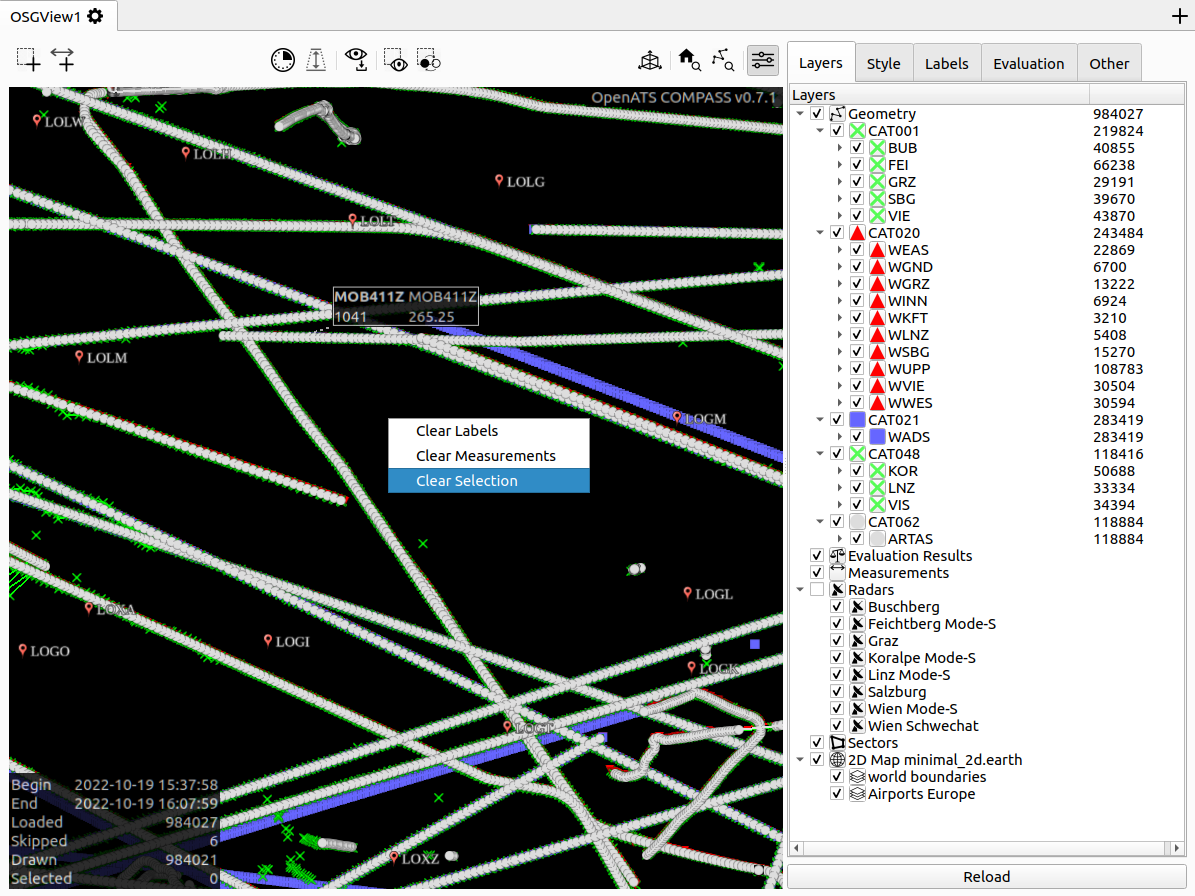
\includegraphics[width=19cm,frame]{figures/osgview_quick_operations.png}
  \caption{OSG View quick menu}
\end{figure}

\begin{itemize}
 \item Clear Labels: Remove all labels
 \item Clear Measurements: Remove all measurements
 \item Clear Selection: Clear selection
\end{itemize}

%\subsubsection{Show Associations}

%Of special interest is of the case when association information is present and a 'UTN' group mode is used. Using the Geometry Menu of a layer item which generated the associations (e.g. ARTAS Tracker), the association information can be shown for each target report of the layer.
% 
% \begin{figure}[H]
%     \hspace*{-2.5cm}
%     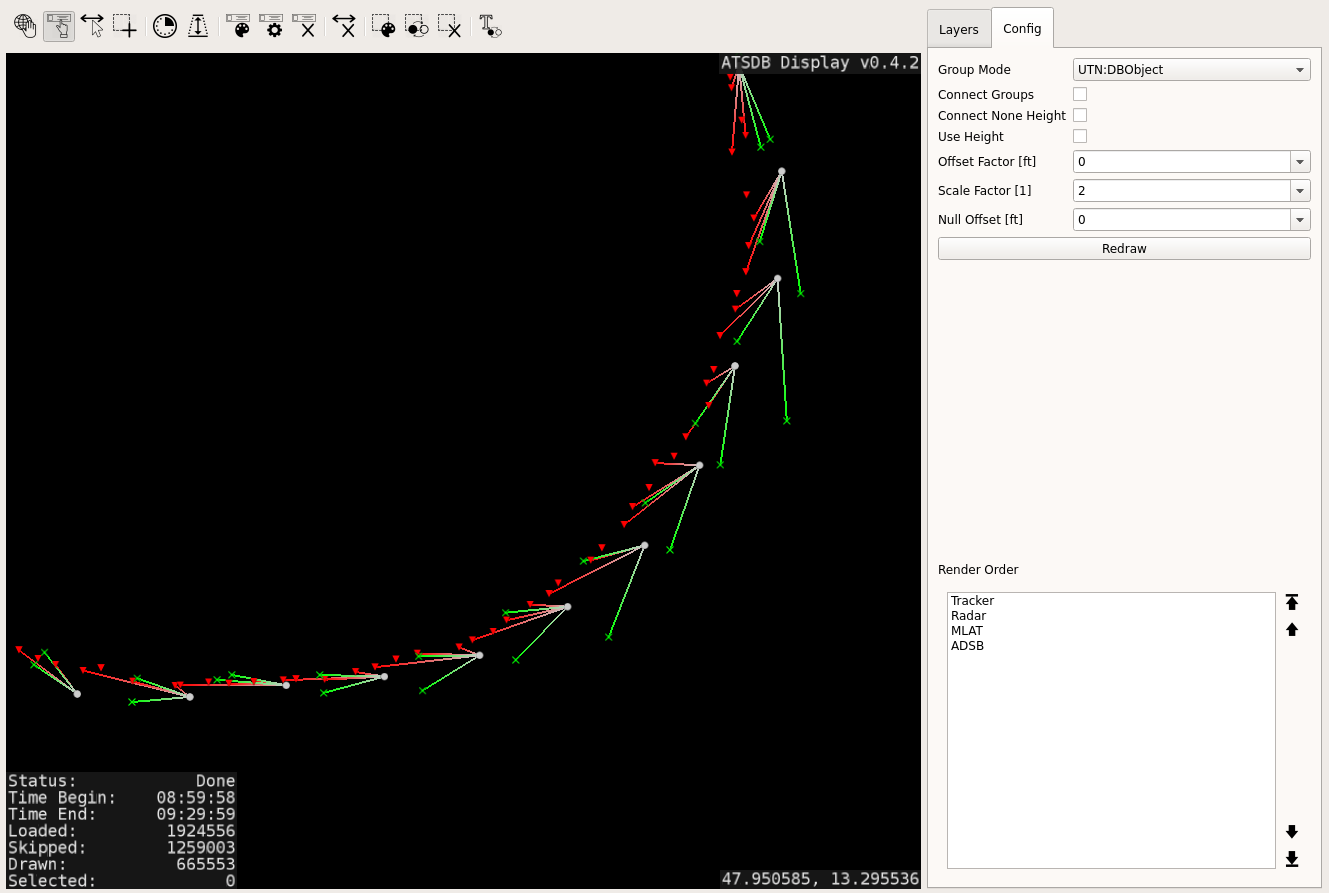
\includegraphics[width=19cm]{figures/osgview_assoc.png}
%   \caption{OSG View show ARTAS association information}
% \end{figure}
% 
% These associations are gradient-coloured from the color of the system track update to color of the associated target report. Additionally, the time window filter can be used to show the timing of the data.
% 
% \begin{figure}[H]
%     \hspace*{-2.5cm}
%     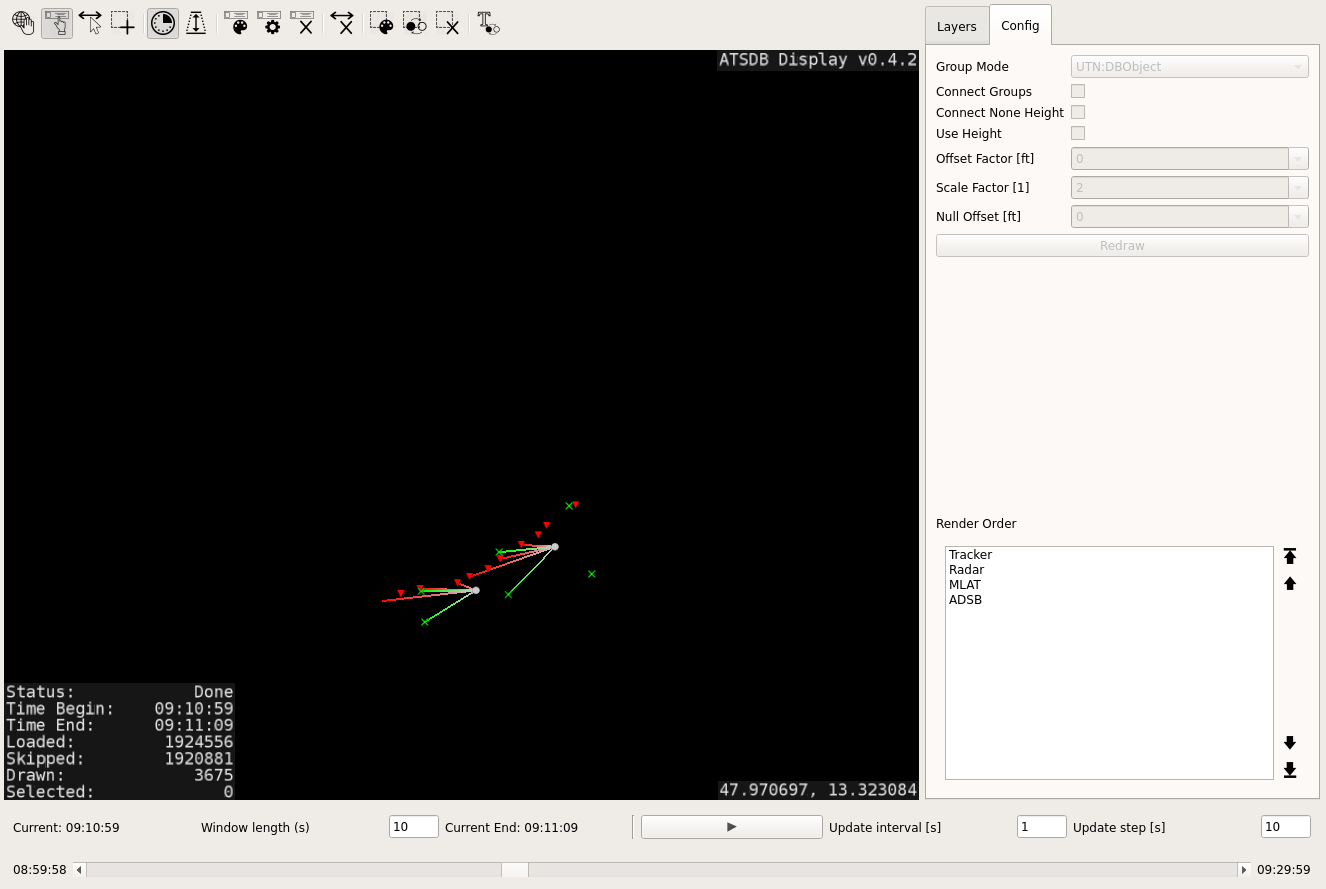
\includegraphics[width=19cm]{figures/osgview_assoc_time_window.png}
%   \caption{OSG View show ARTAS association information in time window}
% \end{figure}

\subsubsection{Selection}
\label{sec:osgview_selection}

Target reports can be selected when the Select mode 
\includegraphics[width=0.5cm,frame]{../../data/icons/select_action.png} is active. If 'Use height' is not checked, select is done as follows:

Simply do a LMB click on a target report or a position on the map to start the selection. Hold and move the mouse to another location to create a red selection rectangle, then release to finalize the selection. \\

Pressing the Escape button during the selection cancels the operations.

\begin{figure}[H]
    \hspace*{-2.5cm}
    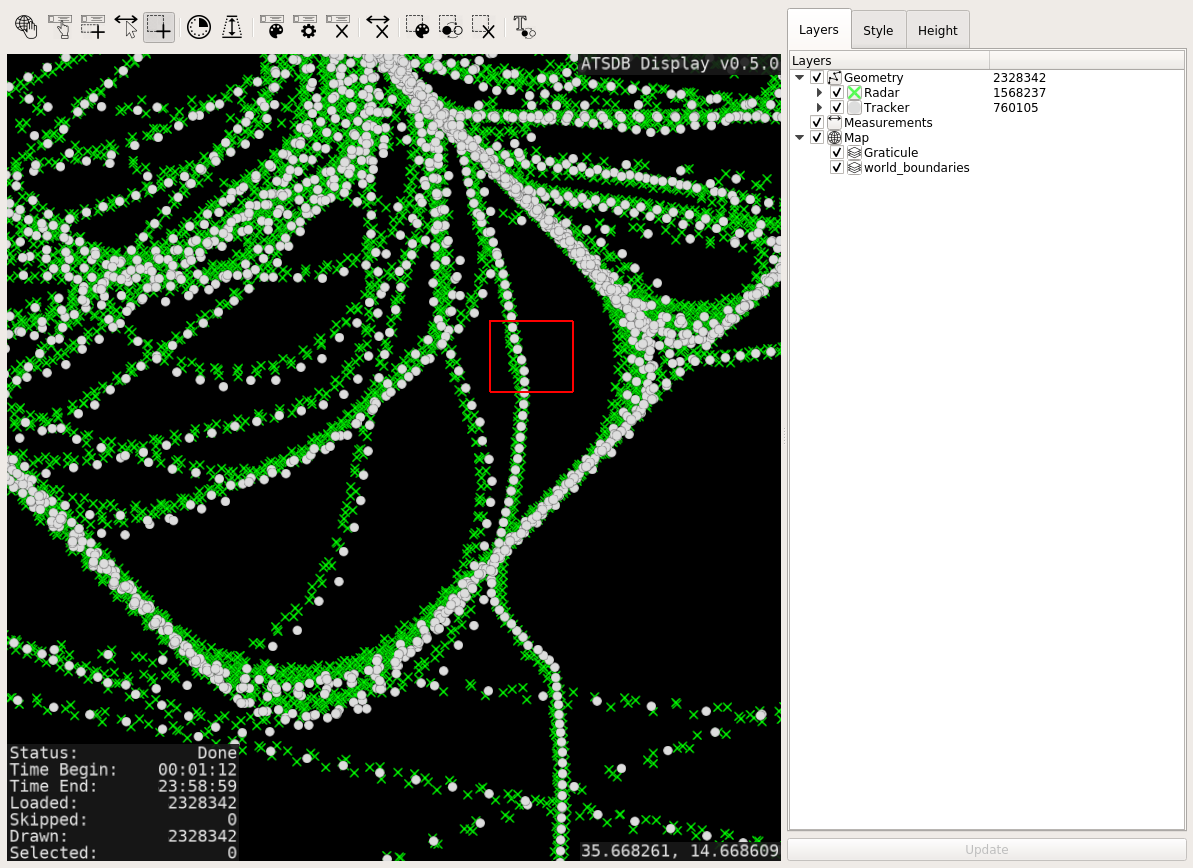
\includegraphics[width=19cm,frame]{figures/osgview_select1.png}
  \caption{OSG View selection}
\end{figure}

When the selection has been done and all target reports in the created latitude/longitude rectangle are selection. This is shown by a different color (yellow by default), and the 'Selected' counter in the lower-left corner shows the current selection size.

\begin{figure}[H]
    \hspace*{-2.5cm}
    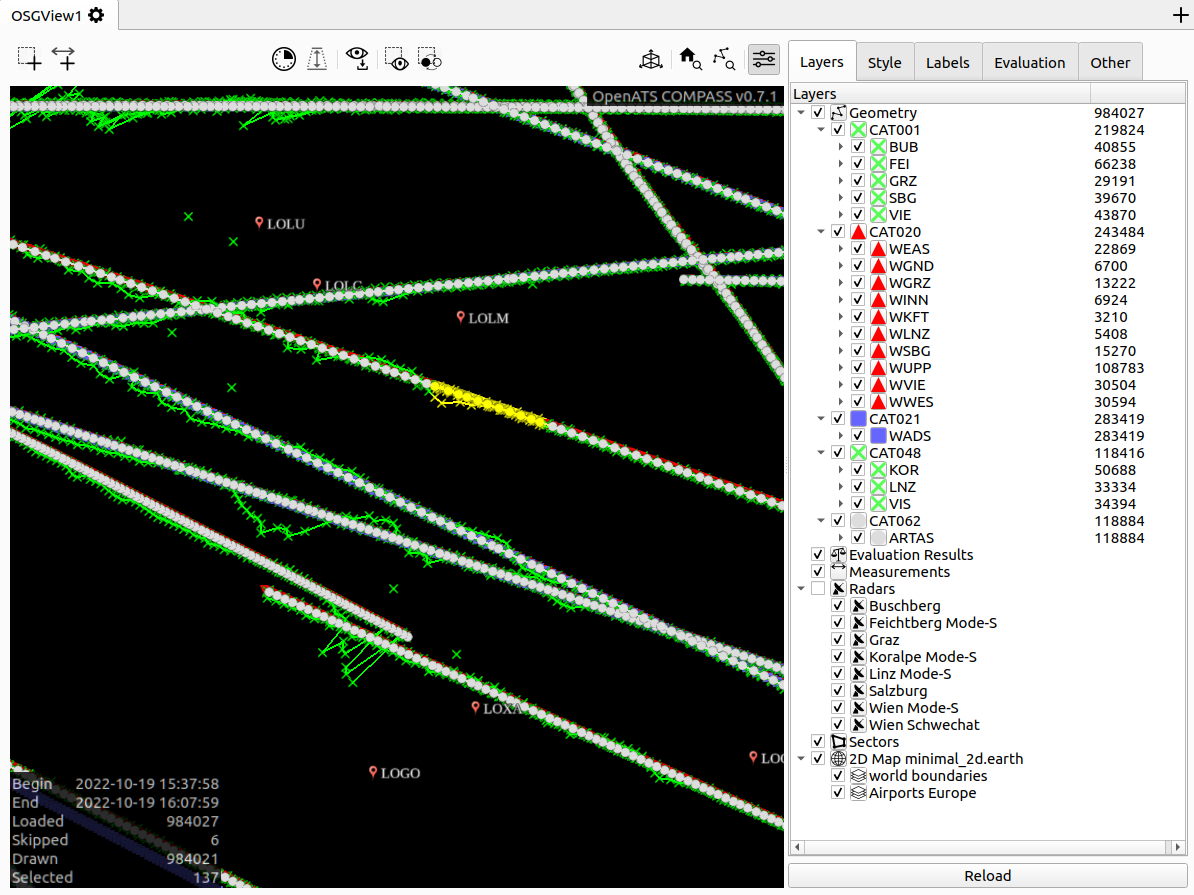
\includegraphics[width=19cm,frame]{figures/osgview_select2.png}
  \caption{OSG View selection done}
\end{figure}

If another selection is done, the previous one is cleared by default. If another selection should be \textit{added} to the current one, hold down the \textbf{Control} key when doing the LMB release.

\begin{figure}[H]
    \hspace*{-2.5cm}
    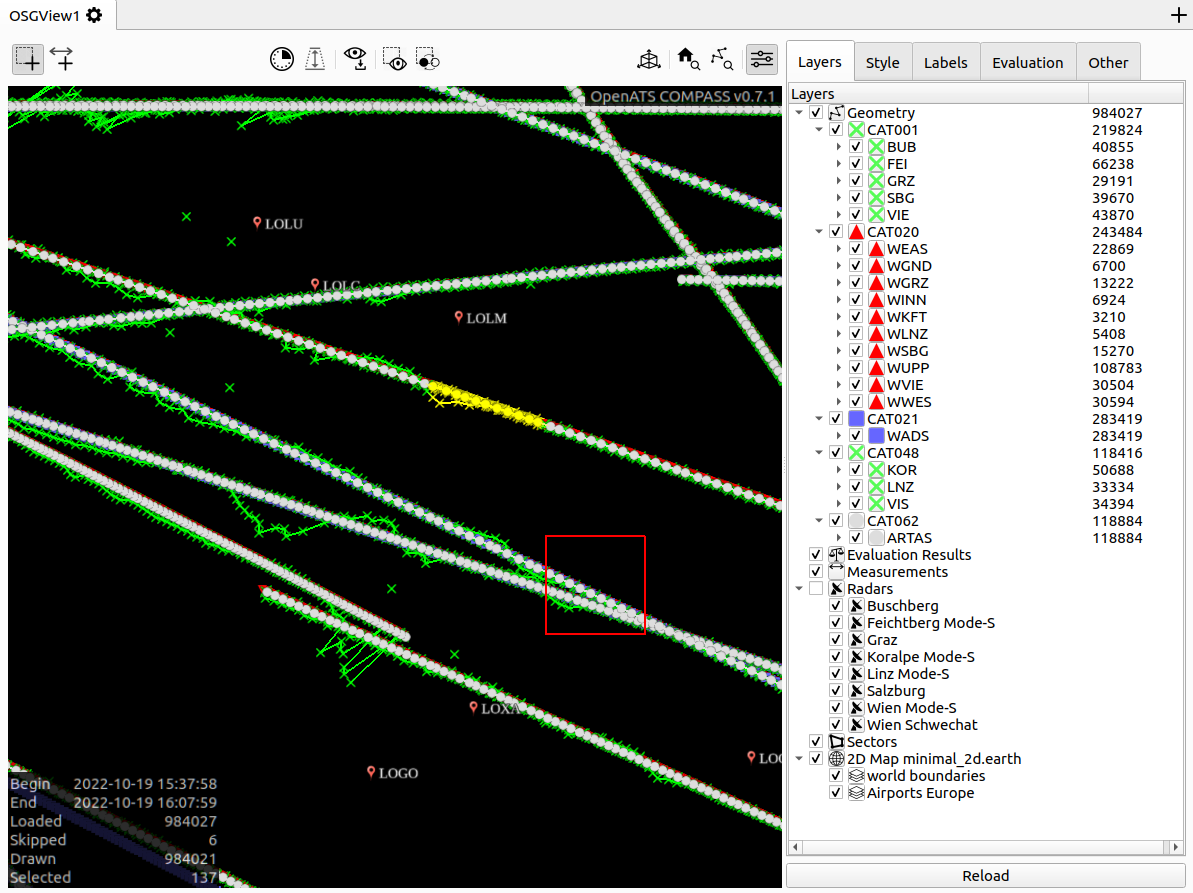
\includegraphics[width=19cm,frame]{figures/osgview_select_add1.png}
  \caption{OSG View selection with adding}
\end{figure}

This adds the target reports within the new red rectangle to the current selecion.

\begin{figure}[H]
    \hspace*{-2.5cm}
    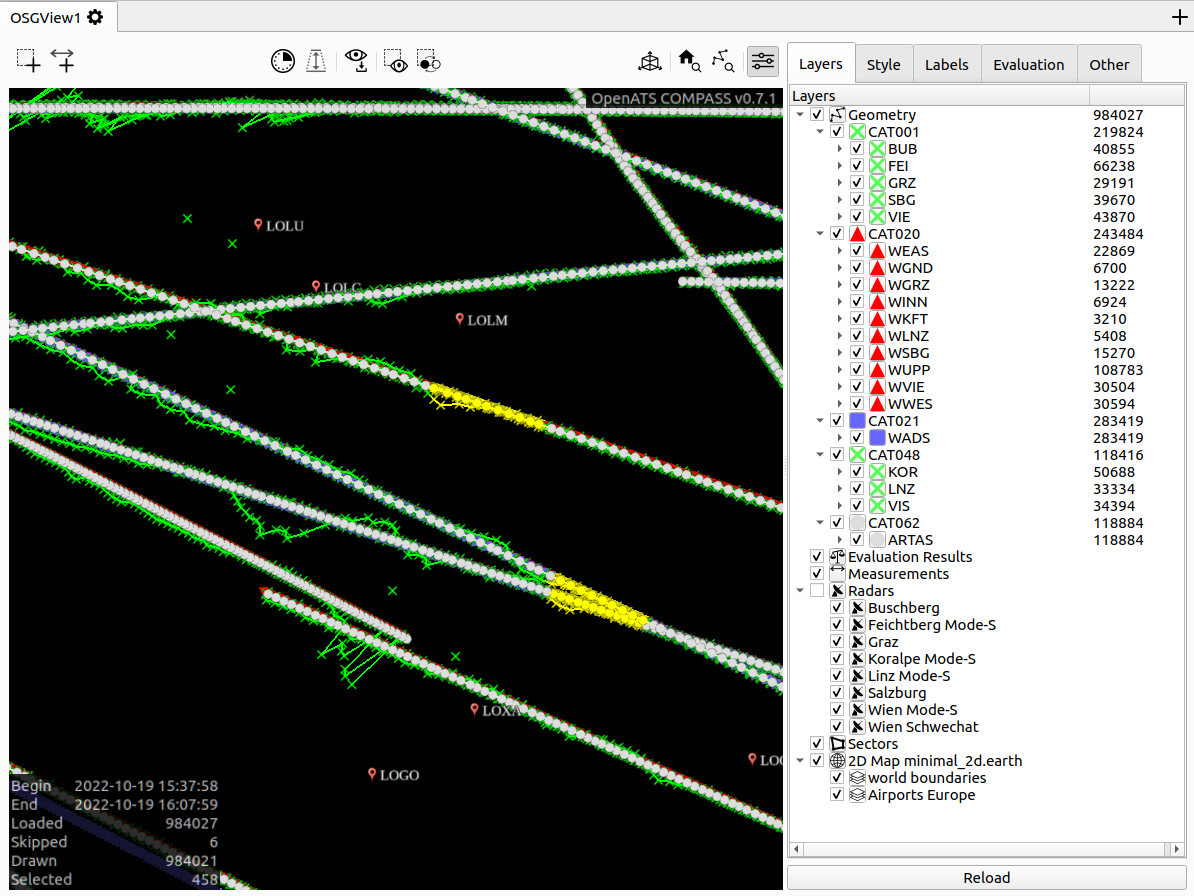
\includegraphics[width=19cm,frame]{figures/osgview_select_add2.png}
  \caption{OSG View selection with adding done}
\end{figure}

If 'Use height' is checked, selection can be done with height information, which is shown as a box. Simply do a LMB click on the map for a target report, and move the cursor to another target report or map location.  \\

If both locations have zero height (map location or no height information in target report), again a rectangle is shown. If one or both locations have a non-zero height, a 3D box is displayed.

\begin{figure}[H]
    \hspace*{-2.5cm}
    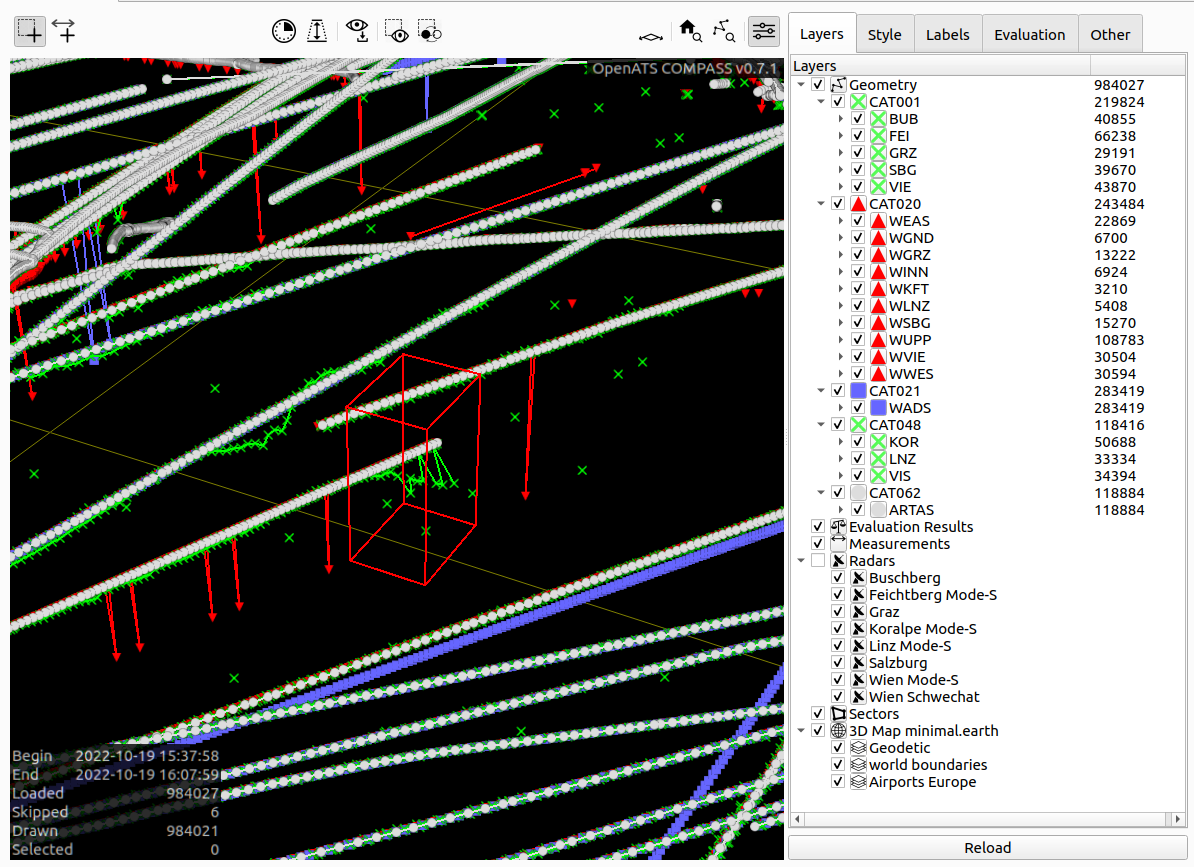
\includegraphics[width=19cm,frame]{figures/osgview_select3d.png}
  \caption{OSG View selection with height}
\end{figure}


\begin{figure}[H]
    \hspace*{-2.5cm}
    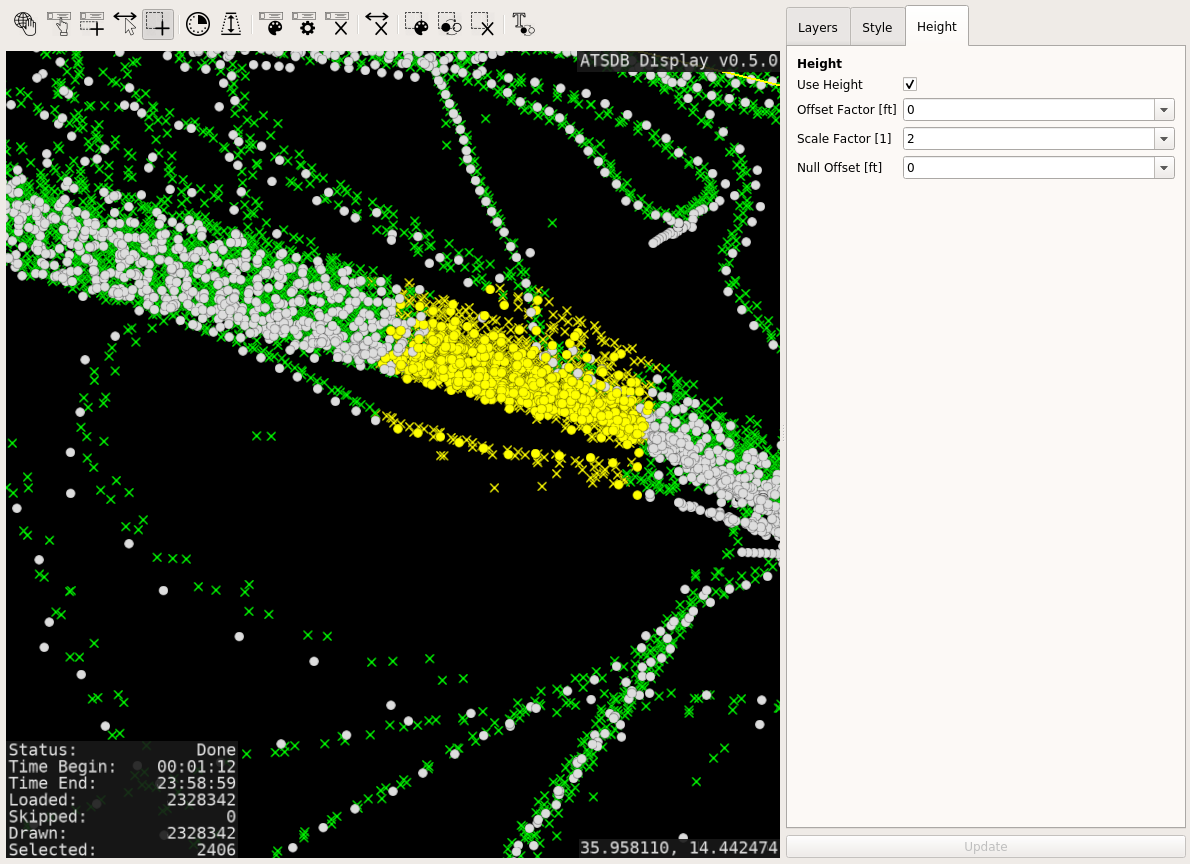
\includegraphics[width=19cm,frame]{figures/osgview_select3d_2.png}
  \caption{OSG View selection with height done}
\end{figure}


\subsubsection{Distance Measurement}
%DONE

Distance measurements can be made when the 'Measure' tool 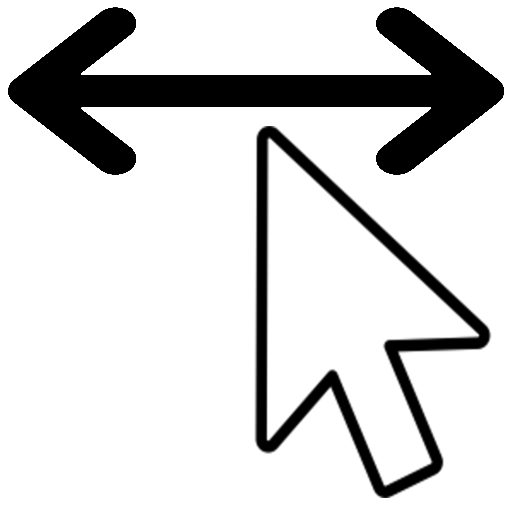
\includegraphics[width=0.5cm,frame]{../../data/icons/measure_action.png} is active. \\

If 'Use height' (section \nameref{sec:others_height}) is not checked, measurements are done as follows: Simply do a LMB click on a target report or a position on the map to start the measurement, then hold the button and drag the mouse to a suitable end position and release the LMB to finish the measurement. \\

Pressing the Escape button during the measurement cancels the operations.

\begin{figure}[H]
    \hspace*{-2.5cm}
    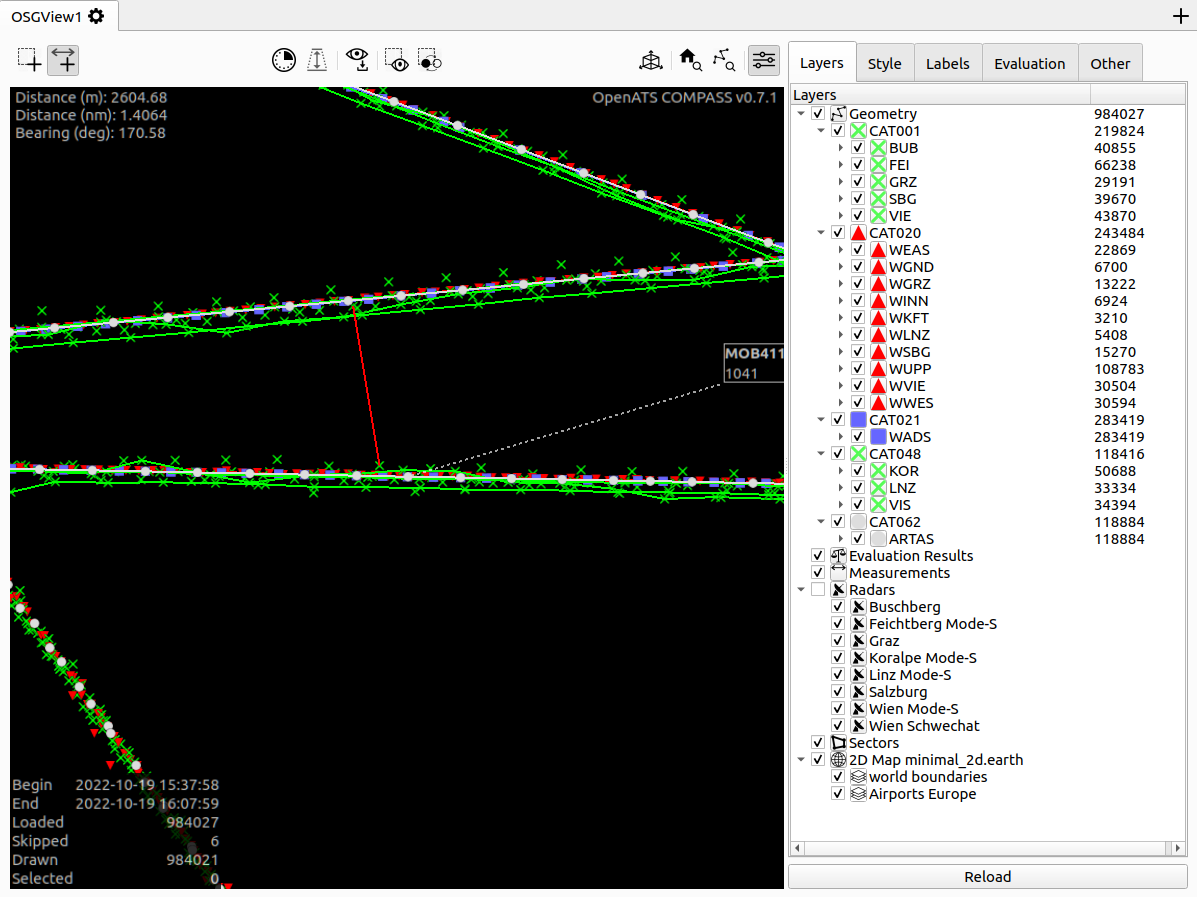
\includegraphics[width=19cm,frame]{figures/osgview_measure1.png}
  \caption{OSG View measurement}
\end{figure}

During measurement, the following information is shown in the top-left corner.

\begin{itemize}
 \item Distance (km): Great-circle distance using the haversine formula, in meters or kilometers.
 \item Distance (nm): Great-circle distance using the haversine formula, in nautical miles.
 \item  Bearing (deg): Bearing from point 1 to point 2, in degrees from true north.
\end{itemize}

\begin{figure}[H]
    \hspace*{-2.5cm}
    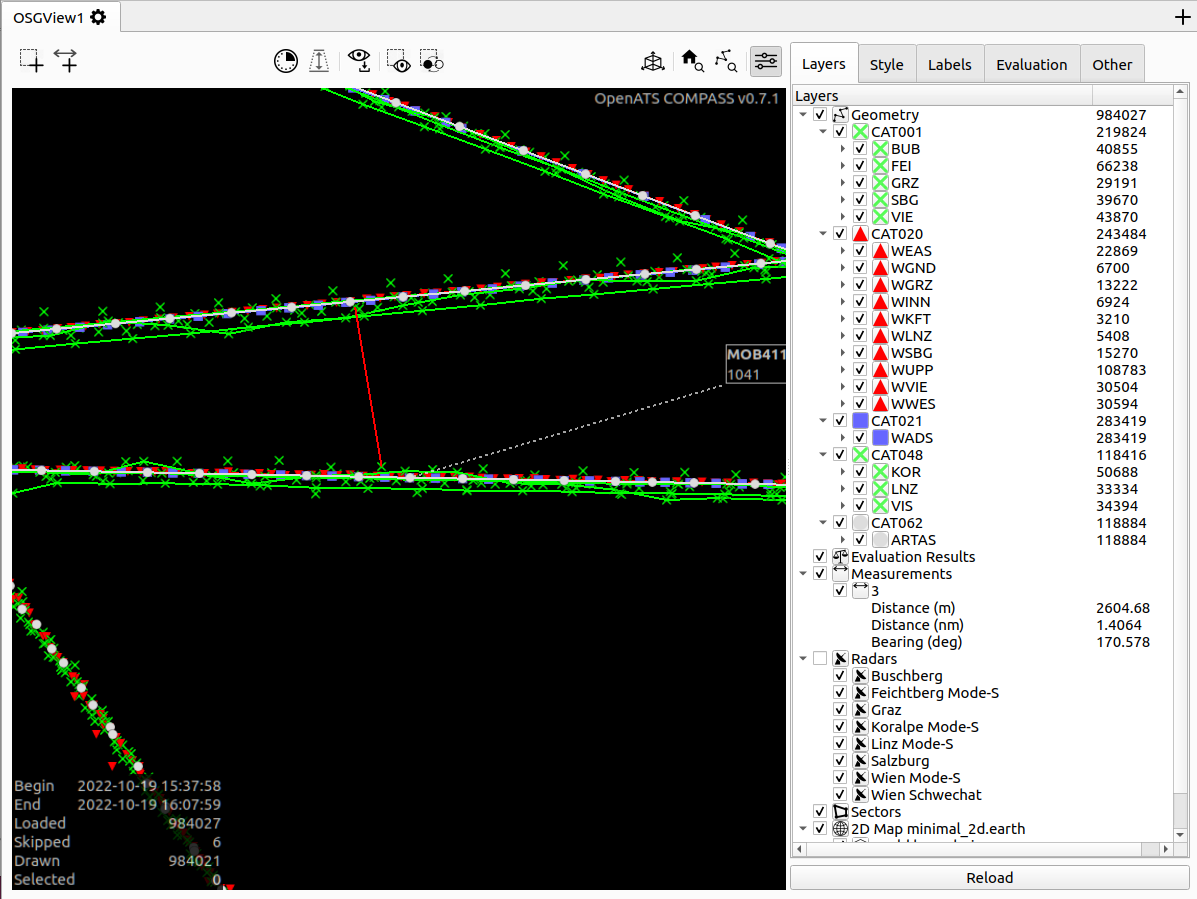
\includegraphics[width=19cm,frame]{figures/osgview_measure2.png}
  \caption{OSG View measurement done}
\end{figure}

If 'Use height' (section \nameref{sec:others_height}) is checked, measurements are calculated in the same way as previously (ground distance), but for each target report with height a connecting line to the respective ground position is displayed. \\

For a measurement between two target reports with height information, the measurement will be displayed as follows:

\begin{figure}[H]
    \hspace*{-2.5cm}
    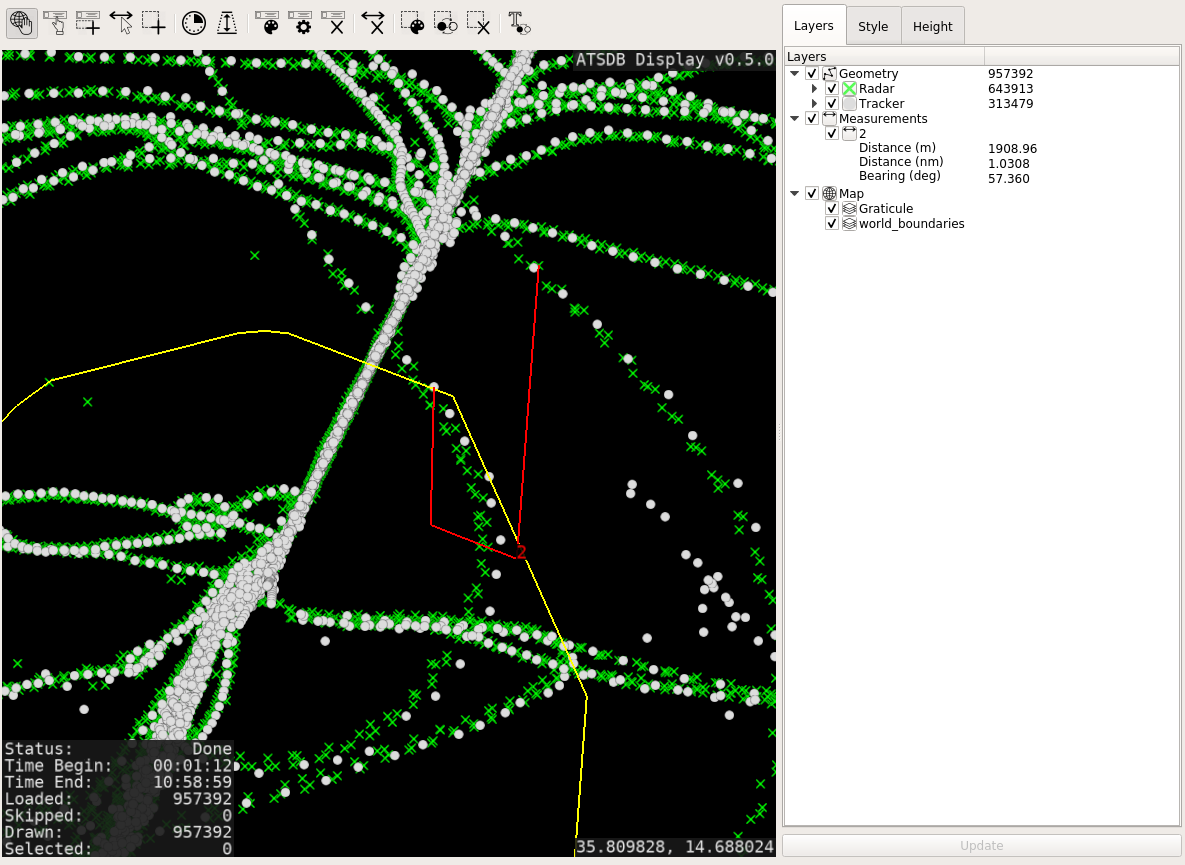
\includegraphics[width=19cm,frame]{figures/osgview_measure3d.png}
  \caption{OSG View measurement with height information}
\end{figure}

%The measurements is shown in the Layers tab, and is identified using a number.

For details about the measurement layer operations please refer to \nameref{sec:osg_measure_ops}. \\

%Please note the the measurement number background color can be set as with the label background color.




\subsubsection{Time Filter}

Once activated using the symbol \includegraphics[width=0.5cm,frame]{../../data/icons/time.png} in the toolbar, the time filter facilitates that only target reports within a specific time window are shown.


\begin{figure}[H]
    \hspace*{-2.5cm}
    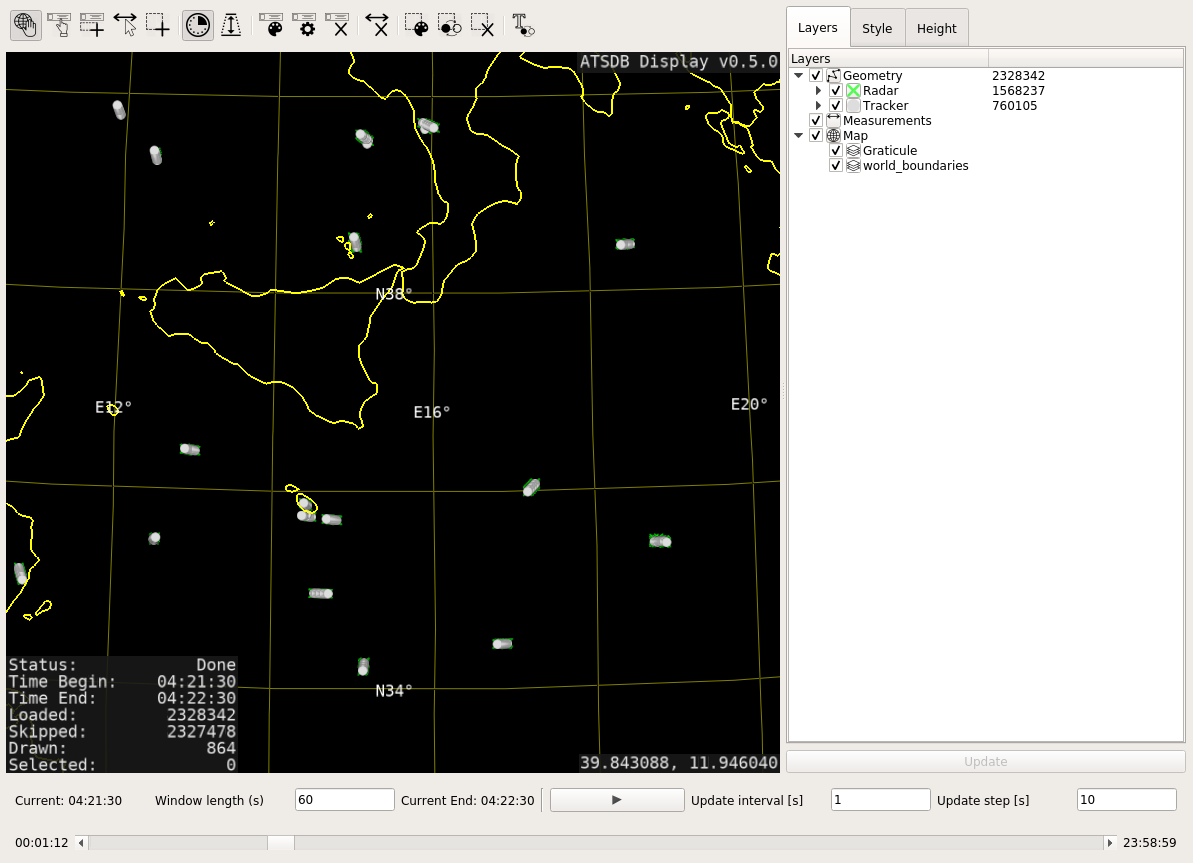
\includegraphics[width=19cm,frame]{figures/osgview_time_filter.png}
  \caption{OSG View time filter}
  \label{fig:osgview_time_filter}
\end{figure}

The following items exist:

\begin{itemize}
 \item Current: The start of the time window
 \item Window length (s): Duration of the display time window
 \item Current End: The end of the time window
 \item Play button: Start/Stop the auto-play mode
 \item Update interval [s]: Auto-play mode update interval
 \item Update step [s]: Auto-play mode update step
 \item Use Opacity: Checkbox and slide to set opacity (older target reports are made transparent)
 \item Scrollbar: Manual time-scrolling
\end{itemize}
\ \\

During usage of the time filter, most changes in the Configuration panel are not available (except for changes in the Layers tab and current style). \\

Please \textbf{note} that the time filter automatically deactivated if a re-load is triggered.

\subsubsection{Depth Check}

Once activated using the symbol \includegraphics[width=0.5cm,frame]{../../data/icons/depth.png} in the toolbar, during drawing it is checked wether data is occluded in the depicted scene. E.g. if target reports are 'below ground', they are not shown.

\begin{figure}[H]
    \hspace*{-2cm}
    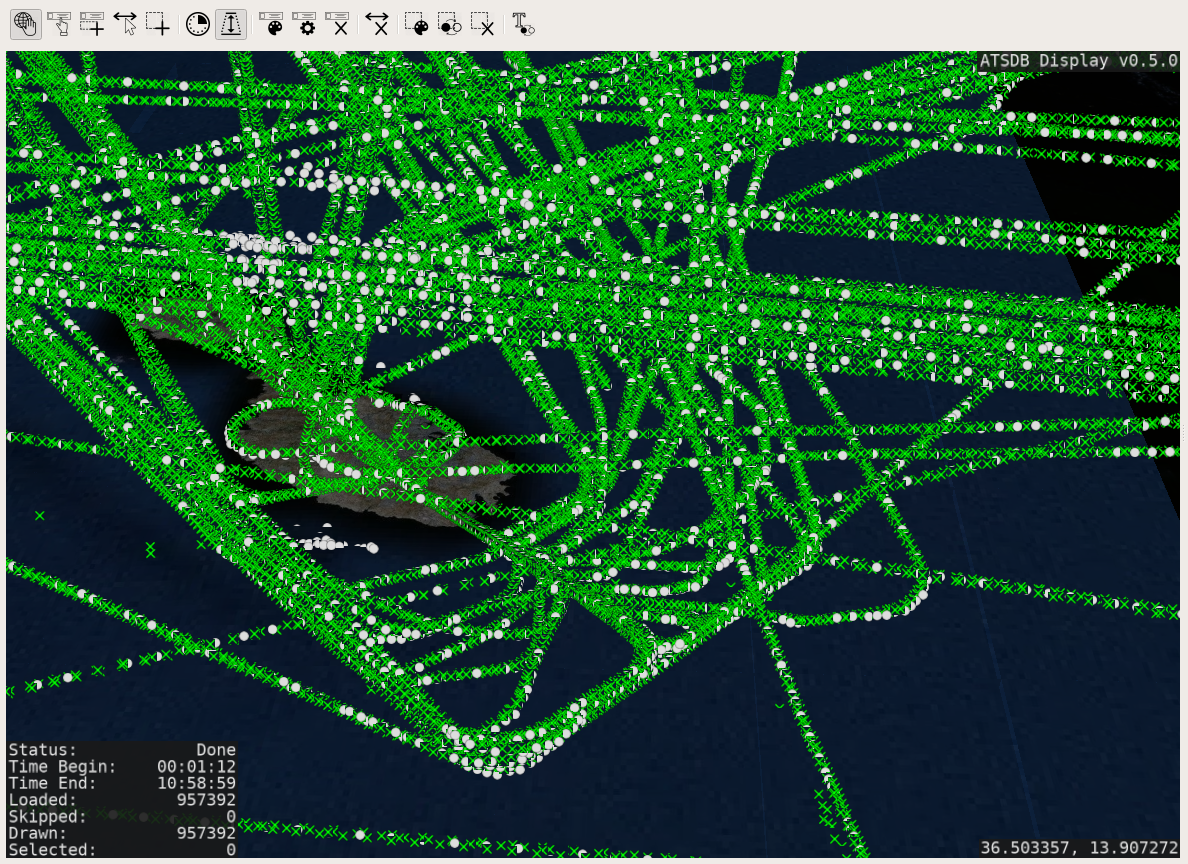
\includegraphics[width=18cm,frame]{figures/osgview_depth_check.png}
  \caption{OSG View depth check}
\end{figure}

Please note that if the display check is activated for geometry without height display, bad rendering can occur. For this reason, this mode is only recommended for geometry display with height and is disabled in 2D display mode.

\subsubsection{Save View Point}

The current filter configuration and viewed position can be saved as a new view point using the symbol \includegraphics[width=0.5cm,frame]{../../data/icons/vp_save.png} in the toolbar. When clicked, a name of the view point has to be entered by the user. 

% \subsubsection{Data Label Deletion}
%
% All existing labels can be deleted using the symbol \includegraphics[width=0.5cm,frame]{../../data/icons/label_delete.png} in the toolbar.
%
% \subsubsection{Measurement Deletion}
%
% All existing measurements can be deleted using the symbol \includegraphics[width=0.5cm,frame]{../../data/icons/measurement_delete.png} in the toolbar.
%
% \subsubsection{Selection Color}
%
% The color for selection highlighting can be configured using the symbol \includegraphics[width=0.5cm,frame]{../../data/icons/select_color.png} in the toolbar.

\subsubsection{Show Only Selected}

When using the symbol 
\includegraphics[width=0.5cm,frame]{../../data/icons/select_show.png} in the toolbar, only the selected data is shown.

\subsubsection{Selection Invert}

The selection can be inverted using the symbol \includegraphics[width=0.5cm,frame]{../../data/icons/select_invert.png} in the toolbar.

% \subsubsection{Selection Deletion}
%
% The selection can be erased using the symbol \includegraphics[width=0.5cm,frame]{../../data/icons/select_delete.png} in the toolbar.
%
% \subsubsection{Overlay Text Color Invert}
%
% The overlay text color can be toggled between black on white or white on black using the symbol \includegraphics[width=0.5cm,frame]{../../data/icons/text_invert.png} in the toolbar. Depending on the map background one or the other is more suitable.

\subsubsection{Switch Map Dimensions}

The display modes can be switched using the symbol \includegraphics[width=0.5cm,frame]{../../data/icons/3d.png} or \includegraphics[width=0.5cm,frame]{../../data/icons/2d.png} in the toolbar, or by pressing the D-key. 

\subsubsection{Zoom to Home}

The currently viewed area can be set to encompass all data in the database using the symbol \includegraphics[width=0.5cm,frame]{../../data/icons/zoom_home.png} in the toolbar.

\subsubsection{Zoom to Loaded Data}

The currently viewed area can be set to encompass all currently loaded data using the symbol \includegraphics[width=0.5cm,frame]{../../data/icons/zoom_geometry.png} in the toolbar.

